% !TEX root = paper.tex
% !TEX encoding = UTF-8 Unicode

\begin{figure}
\begin{center}
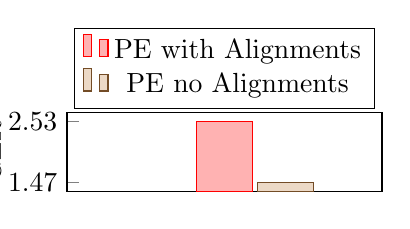
\begin{tikzpicture}[trim left={(-0.5,0)},trim axis right]
\begin{axis}[scale only axis=true, width=40mm, height=10mm,
    ybar,
    enlargelimits=0.15,
    legend style={at={(0.5,1.05)},anchor=south},
   ylabel={GER},
   %xlabel={Post-Editor},
   % symbolic x coords={PE0,PE1,PE2,PE3,PE4,PE5,PE6},
    xtick={0},
    ytick={1.47,2.53},
    xticklabels={""},
	xtick pos=left,
	ytick pos=left,
	ylabel shift={-0.15cm},
    %xtick=data,
    %nodes near coords,
    %nodes near coords align={vertical},
    bar width=20pt
    ]

\addplot 
	coordinates {};
\addplot coordinates { (1,2.53)};
\addplot coordinates { (1,1.47)};

%\addplot[red,sharp plot,update limits=false] 
%	coordinates {(-1,6.1) (8,6.1)};
	%node[above] at (axis cs:3,6.1) {Unedited MT};
	
%%\addplot coordinates {(tool8,1) (tool9,1) (tool10,1)};
\legend{PE with Alignments,PE no Alignments}
\end{axis}
\end{tikzpicture}
\caption{Mean adequacy gain to effort ratio (GER) values for segments post-edited with alignment and without alignment. Effort is measured by pause to word ratio (PWR).}
\label{fig:mean_ger}
\end{center}
\end{figure}
